\begin{figure}[h!]
  \begin{center}
    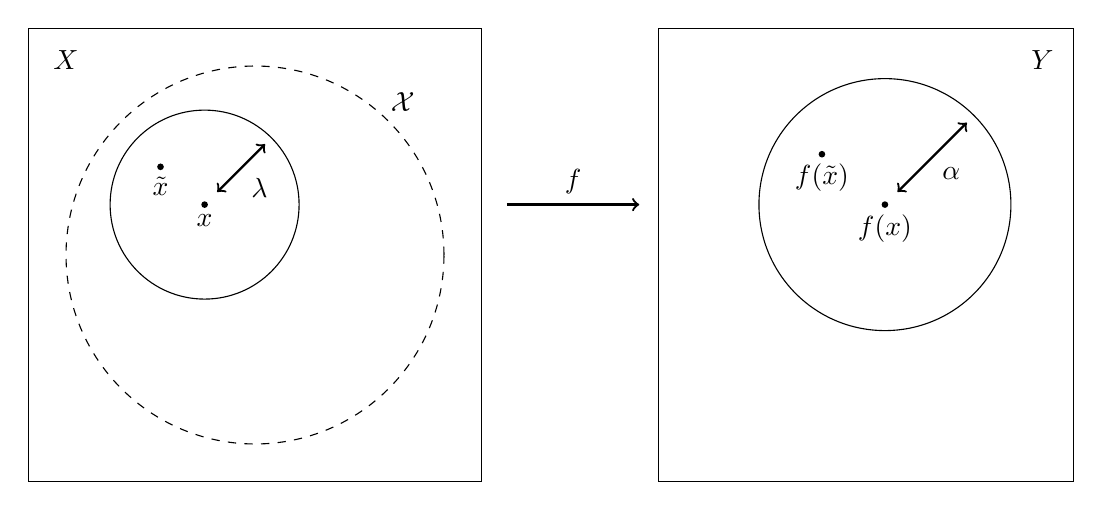
\begin{tikzpicture}[scale=.8]
      \node (X) at (-3, 3.1) {$X$};
      \node (Y) at (12.5, 3.1) {$Y$};

      \draw (-3.6, -3.6) rectangle (3.6, 3.6);
      \draw (6.4, -3.6) rectangle (13, 3.6);

      \fill (-0.8, 0.8) circle (1.5pt);
      \node[below] (x) at (-0.8, 0.8) {$x$};

      \fill (-1.5, 1.4) circle (1.5pt);
      \node[below] (xt) at (-1.5, 1.4) {$\tilde{x}$};

      \fill (10, 0.8) circle (1.5pt);
      \fill (9.0, 1.6) circle (1.5pt);
      \node[below] (y) at (10, 0.8) {$f(x)$};
      \node[below] (yt) at (9.0, 1.6) {$f(\tilde{x})$};

      \draw[dashed] (0, 0) ellipse (3cm and 3cm) node[above right, xshift=1.6cm, yshift=1.7cm] {$\mathcal{X}$};
      \draw[] (-0.8, 0.8) ellipse (1.5cm and 1.5cm);
      \draw[<->, thick] (-0.6, 1) -- ++(0.76, 0.76) node[midway, below right] {$\lambda$};
      \draw[] (10, 0.8) ellipse (2cm and 2cm);
      \draw[<->, thick] (10.2, 1) -- ++(1.1, 1.1) node[midway, below right] {$\alpha$};
      \draw[->, thick] (4, 0.8) -- (6.1, 0.8) node[midway, above] {$f$};
    \end{tikzpicture}
  \end{center}
  \captionsetup{justification=centering}
  \caption{
    \pt{Função $f : \mathcal{X} \to Y$ $(\alpha, \lambda)$-limitada em $x$.}
    \en{Function $f : \mathcal{X} \to Y$ which is $(\alpha, \lambda)$-bounded at $x$.}
  }
\end{figure}
